\section{Adaptive Precision Block-Jacobi Preconditioning} \label{2017-adaptive-block-jacobi:sec:adaptive}
The main goal of this work is to assess the potential benefits of a specialized
version of a block-Jacobi preconditioner that selectively stores part of its
data at low precision---a technique that reduces the memory access volume 
during the
application of a block-Jacobi preconditioner. Concretely, we employ three
precision formats: (1) 16-bit, half precision arithmetic (\fph); 
(2) 32-bit, single precision arithmetic (\fps); and 
(3) 64-bit, (full) double precision arithmetic (\fpd).
The \fps and \fpd roughly correspond to the two \textsc{ieee}
standards that are currently supported by practically all commodity processors
used in everything from desktop systems to high-performance servers. 
On the other hand, \fph has only recently received considerable attention 
because of its usefulness in deep learning applications, and hardware support 
for
this format is now included in the most recent many-core architectures from 
NVIDIA.

For our experiments, we use a PCG Krylov solver to expose the
effects of storing parts of a block-inverse preconditioner at a reduced 
precision.
Before we introduce our preconditioning scheme and the strategy for selecting 
the
appropriate storage format, we note that, for the type of systems that can be
tackled using a CG method, the diagonal blocks of $A$ in the preconditioner $D$ 
are all
symmetric. Therefore, a significant amount of storage (and data transfer cost)
can already be saved by explicitly storing only the lower or upper triangular
part of each block. We also recognize that some computational cost can be saved
by exploiting the symmetry and positive definiteness information of these
diagonal blocks. However, 
as these two cost-saving techniques are orthogonal to those we propose, we 
refrain
from mixing the distinct strategies.

In general, the design of a block-Jacobi preconditioner with adaptive precision 
is based on
the following observations. 
\begin{enumerate} 
	\item In the preconditioner matrix, $D$, each one of the blocks, $D_i$, is 
	independent. 
	\item Except for cases where the iterative solver converges quickly, 
	the overhead incurred by determining an appropriate 
	storage format for the preconditioner (before the iteration commences) 
	is irrelevant. 
	\item The application of each block, $D_i$,
	(i.e., multiplication with the inverse block, $\hD_i$)
	should be done with care to guarantee
	``enough'' precision in the result. 
        As we will show in Section~\ref{2017-adaptive-block-jacobi:sec:erroranalysis}, the accuracy of
this application is largely determined by the condition number of $D_i$
with respect to inversion, denoted hereafter as $\kappa_1(D_i) =
\|D_{i}\|_1 \|D_{i}^{-1}\|_1 = \|D_{i}\|_1 \|\hD_{i}\|_1$,~\cite{GVL3}. 
\end{enumerate} 
Armed with these observations, we propose the following adaptive precision
block-Jacobi preconditioner: 
\begin{enumerate} 
	\item Before the iteration
	commences, the inverse of each block, $D_i$, is computed explicitly using 
	\fpd: 
	$D_i \rightarrow \hD_i$. We note that even if $D_i$ is
	sparse, its inverse, $\hD_i$, is likely a dense matrix. For this reason, we 
	store
	the inverse, $\hD_i$, following the conventional column-major order using
	$m_i\times m_i$ real numbers. 
	\item At the same stage (i.e., before the
	iteration),
	we compute $\kappa_1(D_i) = \kappa_1(\hD_i) =  \|D_{i}\|_1 \|\hD_{i}\|_1$
        and we note
	that, given $\hD_i$ is explicitly available, computing
	$\kappa_1(D_i)$ is straightforward and inexpensive compared with the
	inversion of the block. 
	\item In principle, we store $\hD_i$, which was computed in \fpd, in the
	format determined by its condition number---truncating the entries of the
	block if necessary---as: 
	\begin{equation} \label{2017-adaptive-block-jacobi:eqn:thresholds} \left\{
	\renewcommand{\arraystretch}{1.3} \begin{array}{l} \mathrm{\fph \quad
		if}~\tau_h^L < \kappa_1(D_i) \leq \tau_h^U,\\ \mathrm{\fps \quad
		if}~\tau_s^L < \kappa_1(D_i) \leq \tau_s^U,~\mathrm{and}\\ \mathrm{\fpd
		\quad otherwise}, \end{array} \right. 
	\end{equation} 
	with $\tau_h^L = 0$	and $\tau_h^U = \tau_s^L$. As we will discuss in 
	Section~\ref{2017-adaptive-block-jacobi:sec:erroranalysis}, the
	values for the bounds $\tau_h^U$ and $\tau_s^U$ are selected by taking into
	account the unit roundoff for each format: $u_h \approx 4.88e-04$ for half 
	precision, $u_s \approx 5.96e-08$ for 
	single precision, and $u_d\approx 1.11e-16$ for double precision. 
	\item During the iteration, we recover the block $\hD_i$ stored in the 
	corresponding
	format in memory, transform its entries to \fpd once in
	the processor registers, and apply it in terms of a \fpd~\gemv
	to the appropriate entries of $r_{k+1}$ to produce those of $z_{k+1}$.
	This is a memory bandwidth-bound operation, and, therefore, its cost is 
	dominated
	by the overhead of recovering the data for the preconditioner matrix and the
	vectors from memory (i.e., MEMOPS). Thus, we can expect that in
	practice the FLOPs will be completely ``amortized'' (i.e., overlapped) with
	the data transfers. 
\end{enumerate}

\begin{figure}[t] \begin{center}
		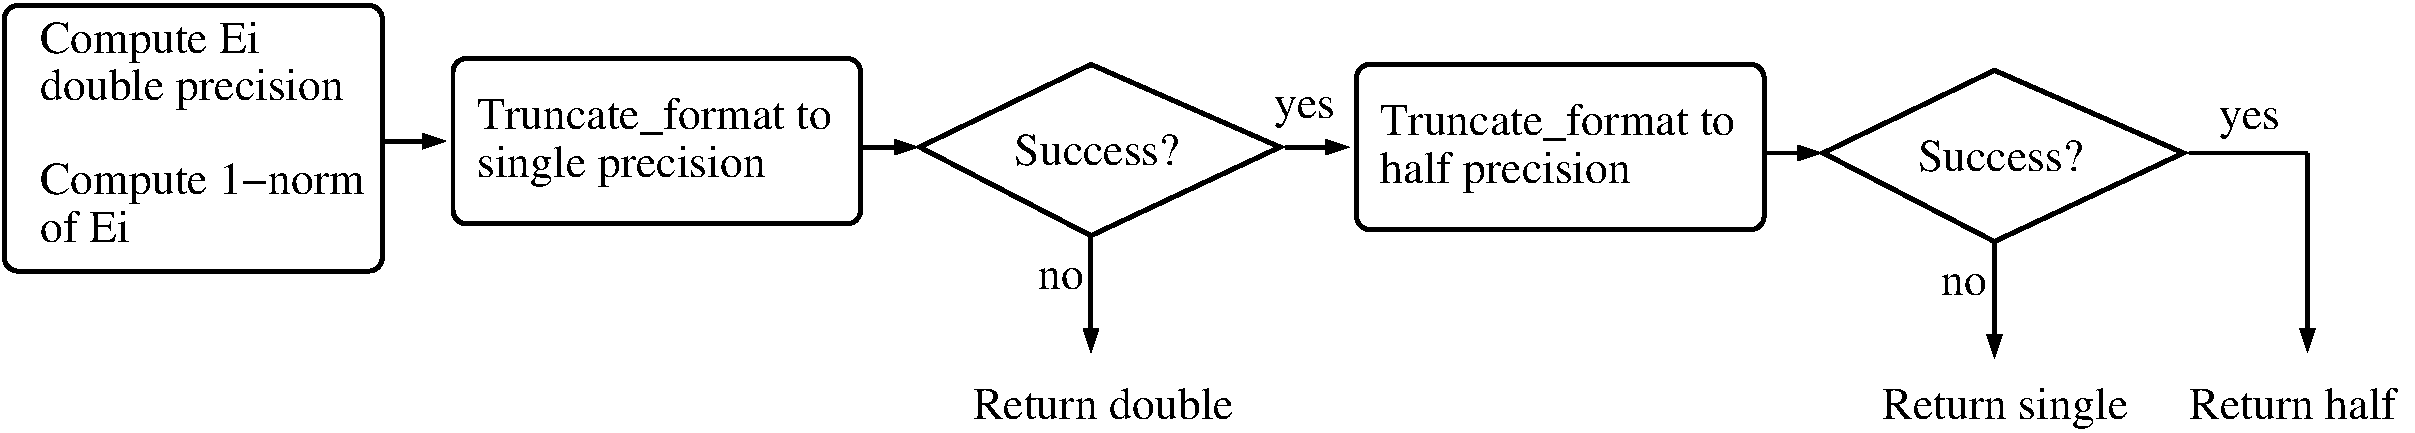
\includegraphics[width=\textwidth]{plots/control-flow}
		\caption{Control flow for deciding whether or not to select a reduced
			format.} \label{2017-adaptive-block-jacobi:fig:control-flow} \end{center} 
		\end{figure}

\begin{figure}[t] \begin{center} \begin{minipage}{\textwidth}
			\lstinputlisting[language=matlab,caption=,]{code/adaptive.m}
		\end{minipage} \caption{Details of the procedure for deciding whether 
		or not to select a
			reduced format.} \label{2017-adaptive-block-jacobi:fig:adaptive} \end{center} 
		\end{figure}

The truncation procedure for converting \fpd data to a reduced precision format 
requires
some care to deal with overflows/underflows and their consequences, as 
described below.
\begin{itemize} 
	\item The truncation of a ``large'' (in magnitude) value in
	$E_i$, represented in \fpd, can produce an overflow because the number
	is too large to be represented in the reduced format, resulting in an 
	``Inf''
	value in that format. In those cases, we can either discard the use of the
	reduced format for the complete block $E_i$ or replace the truncated value 
	with
	the largest number (in magnitude) representable in that format (e.g., for
	positive values, $65,504$ in \fph and about $3.40e+38$ in \fps). 
	\item Conversely, the truncation of a ``small'' (in	magnitude) value, 
	in \fpd, may yield an underflow that returns a value that
	is~zero. This can turn a nonsingular matrix $\hD_i$ into a singular matrix. 
	For
	example, if all entries of $\hD_i$ are below the minimum representable 
	number in
	the reduced format, the result of truncation will produce a block that 
	comprises
	only zeros, and the preconditioned solver will not converge. This could be 
	mitigated to some extent by scaling all the values of the block. 
	Furthermore, even
	if some of the entries are nonzero the truncated representation of $\hD_i$ 
	may
	still become ill-conditioned, thereby causing numerical difficulties for 
	the convergence.
	In order to avoid this issue, we propose checking the condition number of 
	the
	truncated representation and not using the corresponding reduced
	precision if it is above the relevant threshold, $\tau_{\kappa}$. 
\end{itemize} 

Figure~\ref{2017-adaptive-block-jacobi:fig:control-flow} summarizes the global precision
selection process, and the pseudocode in Figure~\ref{2017-adaptive-block-jacobi:fig:adaptive} provides a
practical implementation of the truncation procedure and the various 
thresholds---taking $E_i$ and $\kappa_1(E_i)$ as inputs. The routine 
given in the pseudocode,~{\tt \small force\_reduction}, simply truncates the 
\fpd block to a reduced format. The rest of the code uses several metrics
to determine whether the use of the reduced format is safe.

